\documentclass[12pt]{article}

\usepackage[left=2.5cm,right=2cm,top=2cm,bottom=2cm]{geometry}
\setlength{\parindent}{0mm}

\usepackage{float}

\usepackage{parskip}
\usepackage[document]{ragged2e}
\usepackage{babel}
\usepackage[utf8]{inputenc}
\usepackage{amsmath,amsthm,mathtools}
\usepackage{amsfonts,amssymb,latexsym}
\usepackage{enumerate}
\usepackage[dvips,usenames]{color}
\definecolor{RojoAnayelRey}{rgb}{1,.25,.25}
\usepackage{tikz}
\usepackage[bookmarks=true,
            bookmarksnumbered=false, % true means bookmarks in 
                                     % left window are numbered                         
            bookmarksopen=false,     % true means only level 1
                                     % are displayed.
            colorlinks=true,
            urlcolor=cyan,
            linkcolor=blue]{hyperref}
            
\usepackage[T1]{fontenc}

\title{Tarea evaluable: Análisis de Componentes Principales}

\author{David Cabezas Berrido}

\date{}

\begin{document}
\maketitle
\tableofcontents

\pagebreak

He elegido el \textbf{Problema 2}, sobre las puntuaciones de 13 empresas en 8 indicadores económicos. 
\vspace{-7mm}
\section{Carga, análisis exploratorio y preparación de los datos}

\subsection{Carga y tratamiento de valores perdidos}

Comenzamos cargando los datos de \textbf{empresas.sav}.

\begin{verbatim}
> library(foreign)
> datos<-read.spss("empresas.sav", to.data.frame = TRUE, reencode="utf-8")
> round(datos,4)

           x1      x2      x3      x4      x5      x6      x7      x8
1      0.1280  0.9444  2.1667  5.7943  5.4803 11.0963  3.9821  5.7987
2      1.5525  4.2997  4.3333  5.4044  5.3356 11.0115  5.5841  8.1026
3      1.2148  6.8998  6.5000  4.0673  6.8894 24.7631  7.2766 14.3987
4      2.4759  8.6931  8.6667  7.4094  4.1379 31.5858 10.3398 17.8725
5      6.0131 11.2399 10.8333  0.0299 10.0368 10.1698  1.9664  7.5506
6      6.7350 13.1272 13.0000  1.5495  5.8742  6.1346  1.0636  3.9489
7      7.5839 14.8487 15.1667 11.3959  2.7099  6.9551  1.6670  4.7504
8      8.0142 18.1598 17.3333  6.3268  2.5565 41.5239 12.3739 26.2319
9      8.1197 19.5661 19.5000  6.5147  3.4624 31.0378 10.1604 20.1541
10    11.5167 21.7262 21.6667  5.0601  5.9190 43.2783 12.2356 26.5714
11    10.7337 24.1411 23.8333  3.9694  5.5955 11.3741  5.2363  7.3334
12    11.9853 24.8071 26.0000  4.8855  4.8703  9.7093  4.0888  6.8327
13    14.3636 25.4261 28.1667  7.7611  3.5246 34.4364  9.7984 20.4134
14 20023.0000 18.0000 16.0000  8.0000  8.0000 10.0000      NA      NA
\end{verbatim}

Nos informan de que hay 13 empresas y vemos 14 líneas. La última línea
es muy sospechosa: todos sus valores son enteros, tiene dos valores
perdidos y el valor 20023 en la variable X1 (indicador del volumen de
facturación), lo que distorsiona el \texttt{summary} de los datos:
\begin{verbatim}
       x1                  x2                x3               x4            
 Min.   :    0.128   Min.   : 0.944   Min.   : 2.167   Min.   : 0.030     
 1st Qu.:    3.360   1st Qu.: 9.330   1st Qu.: 9.208   1st Qu.: 4.272     
 Median :    7.799   Median :16.424   Median :15.583   Median : 5.599     
 Mean   : 1436.674   Mean   :15.134   Mean   :15.226   Mean   : 5.584     
 3rd Qu.:   11.321   3rd Qu.:21.186   3rd Qu.:21.125   3rd Qu.: 7.186     
 Max.   :20023.000   Max.   :25.426   Max.   :28.167   Max.   :11.396   
                                               
      x5             x6               x7               x8        
 Min.   : 2.557   Min.   : 6.135   Min.   : 1.064   Min.   : 3.949  
 1st Qu.: 3.678   1st Qu.:10.042   1st Qu.: 3.982   1st Qu.: 6.833  
 Median : 5.408   Median :11.235   Median : 5.584   Median : 8.103  
 Mean   : 5.314   Mean   :20.220   Mean   : 6.598   Mean   :13.074  
 3rd Qu.: 5.908   3rd Qu.:31.449   3rd Qu.:10.160   3rd Qu.:20.154  
 Max.   :10.037   Max.   :43.278   Max.   :12.374   Max.   :26.571  
                                   NA's   :1        NA's   :1   
\end{verbatim}

En la variable X1, el tercer cuartil vale 11.321 y la media es
1436.674, debido a que la fila 14 introduce un valor desproporcinado.

Tenemos razones para pensar que las filas que corresponden a las 13
empresas son las 13 primeras, por lo que eliminamos la 14.
\begin{verbatim}
> datos<-datos[-14,]
\end{verbatim}

\subsection{Estudio de la escala y variabilidad de las variables}

Visualizamos ahora el resumen de los datos
\begin{verbatim}
       x1               x2                x3               x4         
 Min.   : 0.128   Min.   : 0.944   Min.   : 2.167   Min.   : 0.030  
 1st Qu.: 2.476   1st Qu.: 8.693   1st Qu.: 8.667   1st Qu.: 4.067  
 Median : 7.584   Median :14.849   Median :15.167   Median : 5.404  
 Mean   : 6.957   Mean   :14.914   Mean   :15.167   Mean   : 5.398  
 3rd Qu.:10.734   3rd Qu.:21.726   3rd Qu.:21.667   3rd Qu.: 6.515  
 Max.   :14.364   Max.   :25.426   Max.   :28.167   Max.   :11.396 
 
       x5               x6               x7               x8        
 Min.   : 2.557   Min.   : 6.135   Min.   : 1.064   Min.   : 3.949  
 1st Qu.: 3.525   1st Qu.:10.170   1st Qu.: 3.982   1st Qu.: 6.833  
 Median : 5.336   Median :11.374   Median : 5.584   Median : 8.103  
 Mean   : 5.107   Mean   :21.006   Mean   : 6.598   Mean   :13.074  
 3rd Qu.: 5.874   3rd Qu.:31.586   3rd Qu.:10.160   3rd Qu.:20.154  
 Max.   :10.037   Max.   :43.278   Max.   :12.374   Max.   :26.571
\end{verbatim}

Observamos que no quedan valores nulos, luego no debemos preocuparnos de
cómo imputarlos.

También podemos usar un boxplot para observar la distribución de cada variable con mayor comodidad.
\begin{verbatim}
> boxplot(datos,main="Análisis exploratorio de datos",
+         xlab="Indicadores económicos",
+         ylab="Distribución de valores",
+         col=c(1:15))
\end{verbatim}
\vspace{-3mm}
\begin{figure}[H]
  \centering
  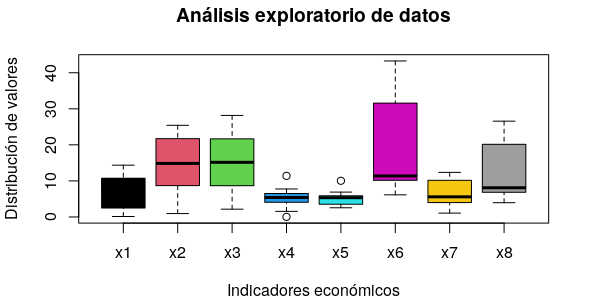
\includegraphics[width=110mm]{imgs/boxplot-analisis}
  \caption{Distribución de las variables}
  \label{fig:boxplot-analisis}
\end{figure}

Observamos que las variables tienen escalas diferentes, por ejemplo el
indicador X6 llega a tomar el valor 40 mientras que los indicadores X4
y X5 no pasan del valor 10. También observamos algunos outliers en los
indicadores X4 y X5. Además, nos percatamos de que algunas
distribuciones son bastante asimétricas: las variables X6, X7 y X8
tienen una mediana muy próxima al primer cuartil, mientras que la
variable X5 la tiene muy próxima al tercer cuartil.

\subsection{Estandarización de los datos}

Los distintos rangos de escalas de las variables nos sugieren que
estas no están estandarizadas, lo corroboramos obteniendo la media y desviación típica de cada columna.

\begin{verbatim}
> round(colMeans(datos),4)
     x1      x2      x3      x4      x5      x6      x7      x8 
 6.9566 14.9138 15.1667  5.3976  5.1071 21.0058  6.5979 13.0738 

> round(apply(datos, 2, sd),4)
     x1      x2      x3      x4      x5      x6      x7      x8 
 4.5451  8.1626  8.4380  2.8238  1.9919 13.7798  4.0307  8.2497 
\end{verbatim}

Observamos que las columnas no tienen media 0 y varianza unidad, por
lo que los datos no están estandarizados. Lo hacemos nosotros.

\begin{verbatim}
> datos_pca<-scale(datos)

> round(colMeans(datos_pca),4)
x1 x2 x3 x4 x5 x6 x7 x8 
 0  0  0  0  0  0  0  0 

> round(apply(datos_pca, 2, sd),4)
x1 x2 x3 x4 x5 x6 x7 x8 
 1  1  1  1  1  1  1  1 
\end{verbatim}

Nos preguntamos que problemas podríamos haber encontrado en el caso de
no hacer la estandarización, y son dos. Para entenderlos, debemos
tener claro el objetivo de PCA: Hallar una base ortonormal de
$\mathbb{R}^8$ (en este caso hay 8 variables) tal que la distribución
esté contenida en la mayor medida posible un subespacio vectorial (de
dimensión lo más pequeña posible) formado por algunos elementos de la
base, de forma que al realizar la proyección perdamos la menor
información posible. El no estandarizar supone dos problemas:
\begin{itemize}
\item El primero es que las
variables tienen distinta escala, por lo que las variables con mayor
escala cobrarían más importancia (comparando con el indicador X6, los
indicadores X4 y X5 están muy cercanos al eje, por lo que la
distribución ``es bastante estrecha'' en estas dimensiones), este
problema lo resolvemos dividiendo los valores por su desviación
típica, para así igualar sus escalas.
\item El segundo problema es que los valores de las variables no están
  centrados en torno al cero, por lo que como mucho podríamos esperar
  que la distribución esté contenida en un subespacio afín y no
  vectorial, resolvemos este problema restando la media de las columnas,
  para trasladar la distribución al origen.
\end{itemize}

\subsection{Análisis de la correlación de las variables} \label{sec:acp}

Primero debemos preguntarnos si tiene sentido hacer un Análisis de
Componentes Principales, en la matriz de correlación observamos altas
correlaciones entre algunas variables: un 97\% de correlación entre
los índices X1 y X2, un 98\% de correlación entre los índices X1 y X3,
un 99\% de correlación entre los índices X6 y X8, y algunas más.

\begin{verbatim}
> round(cor(datos_pca),4) # Matriz de correlación
        x1      x2      x3      x4      x5      x6      x7      x8
x1  1.0000  0.9722  0.9805  0.1028 -0.2575  0.2643  0.2142  0.2988
x2  0.9722  1.0000  0.9940  0.1130 -0.3080  0.3122  0.2933  0.3479
x3  0.9805  0.9940  1.0000  0.1479 -0.3261  0.2984  0.2795  0.3285
x4  0.1028  0.1130  0.1479  1.0000 -0.8409  0.2515  0.2958  0.2294
x5 -0.2575 -0.3080 -0.3261 -0.8409  1.0000 -0.3483 -0.4155 -0.3428
x6  0.2643  0.3122  0.2984  0.2515 -0.3483  1.0000  0.9666  0.9940
x7  0.2142  0.2933  0.2795  0.2958 -0.4155  0.9666  1.0000  0.9632
x8  0.2988  0.3479  0.3285  0.2294 -0.3428  0.9940  0.9632  1.0000
\end{verbatim}

Por tanto, parece que podremos reducir en cierta medida el número de
variables sin perder demasiada información. Nos aseguramos de esto
realizando el Test de Bartlett, debe aplicarse a los datos
normalizados, pero ya lo están.

\begin{verbatim}
> library(psych)
> cortest.bartlett(cor(datos_pca),n=13) # n es el tamaño de muestra
$chisq
[1] 154.2293
$p.value
[1] 2.122684e-19
\end{verbatim}

Observamos un p-valor prácticamente nulo, por lo que rechazamos la
hipótesis nula y concluimos que los datos están correlados, por lo que
procedemos con el Análisis de Componentes Principales.
\subsection{Limpieza de outliers}
Este análisis es muy sensible a outliers, y comprobamos en la Figura
\ref{fig:boxplot-analisis} que las variables X4 y X5 presentan
algunos, que no cambian con la estandarización. Por eso los
sustituimos por la media con el código que mejoramos en la tarea
voluntaria, para realizar justo el número necesario de pasadas en cada
columna que presente outliers.

\begin{verbatim}
outlier<-function(data,na.rm=T){ # Función para limpiar los outliers
  continue<-TRUE
  while(continue){
    H<-1.5*IQR(data)
    data[data<quantile(data,0.25,na.rm = T)-H]<-NA
    data[data>quantile(data,0.75, na.rm = T)+H]<-NA
    continue<-any(is.na(data))
    data[is.na(data)]<-mean(data,na.rm=T)
  }
  data
}
\end{verbatim}
Aplicamos esta función a las dos columnas que presentan outliers.
\begin{verbatim}
> datos_pca[,4]<-outlier(datos_pca[,4])
> datos_pca[,5]<-outlier(datos_pca[,5])
\end{verbatim}

En la Figura \ref{fig:boxplot-outliers} comparamos los datos
estandarizados antes y después de eliminar los outliers. Apreciamos
que la estandarización ha centrado las distribuciones en el 0 y ha
equiparado las escalas de las variables, pero se mantienen los
outliers (comparar boxplot de la izquierda con Figura
\ref{fig:boxplot-analisis}). Eliminar los outliers también ha
desplazado y modificado el grueso de la distribución de estas
variables (comparar el boxplot de la izquierda con el de la derecha
(las cajas azul claro, X4 y oscuro, X5).

\begin{figure}[H]
  \centering
  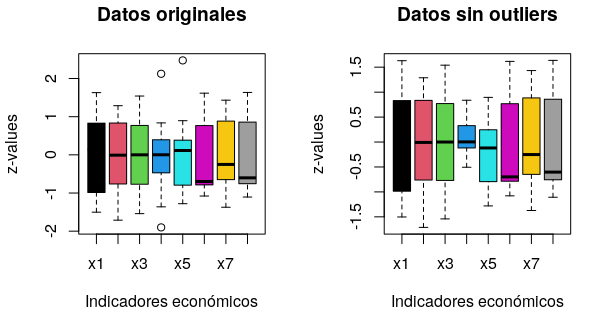
\includegraphics[width=140mm]{imgs/boxplot-outliers}
  \caption{Limpieza de los outliers}
  \label{fig:boxplot-outliers}
\end{figure}

\pagebreak
\section{Análisis de Componentes Principales}

\subsection{Obtención de las componentes principales y sus varianzas explicada y acumulada}

Realizamos el ACP:
\begin{verbatim}
PCA<-prcomp(datos_pca, scale=T, center = T)
\end{verbatim}
En la matriz de rotación, podemos consultar el peso de cada variable en cada componente principal:
\begin{table}[H]
  \centering
\begin{verbatim}
> round(PCA$rotation,4)
       PC1     PC2     PC3     PC4     PC5     PC6     PC7     PC8
x1  0.3576 -0.4467  0.0024 -0.1589  0.4267 -0.6514  0.0017 -0.2023
x2  0.3720 -0.4295  0.0686  0.0104 -0.2191  0.4928  0.4264 -0.4468
x3  0.3713 -0.4320  0.0332 -0.1031 -0.2512  0.1648 -0.4236  0.6278
x4  0.2381  0.2921 -0.5866 -0.7069 -0.0497  0.0709  0.0819 -0.0082
x5 -0.2531 -0.0291  0.6979 -0.6654 -0.0052  0.0393  0.0588  0.0108
x6  0.3994  0.3426  0.2280  0.0299  0.3303  0.3018 -0.5885 -0.3518
x7  0.3857  0.3516  0.2473  0.0768 -0.6673 -0.4484  0.0306 -0.1153
x8  0.4084  0.3197  0.2233  0.1214  0.3873  0.0830  0.5304  0.4776
\end{verbatim}
  \caption{Matriz de cambio de base entre las variables y las
    componentes principales. Contiene las contribuciones de las
    variables a cada componente principal.}
  \label{tab:mat-rot}
\end{table} \vspace{-5mm}
También podemos ver con \texttt{summary} la desviación típica
(\texttt{PCA\$sdev}), la varianza explicada y la acumulada por cada
componente principal:
\begin{verbatim}
> summary(PCA)
Importance of components:
                          PC1    PC2    PC3     PC4     PC5     PC6     PC7     PC8
Standard deviation     2.0461 1.4874 1.1025 0.55772 0.23779 0.10786 0.06953 0.03781
Proportion of Variance 0.5233 0.2765 0.1519 0.03888 0.00707 0.00145 0.00060 0.00018
Cumulative Proportion  0.5233 0.7999 0.9518 0.99069 0.99776 0.99922 0.99982 1.00000
\end{verbatim}

Podemos visualizar estas cantidades utilizando el paquete \texttt{ggplot}.
\begin{verbatim}
library("ggplot2")
> prop_var<- PCA$sdev^2 / sum(PCA$sdev^2)
> ggplot(data = data.frame(prop_var, pc = 1:8),
+        aes(x = pc, y = prop_var, fill=prop_var )) +
+   geom_col(width = 0.3) +
+   scale_y_continuous(limits = c(0,0.6)) + theme_bw() +
+   labs(x = "Componente principal", y= " Proporción de varianza explicada")
\end{verbatim}

\begin{figure}[H]
  \centering
  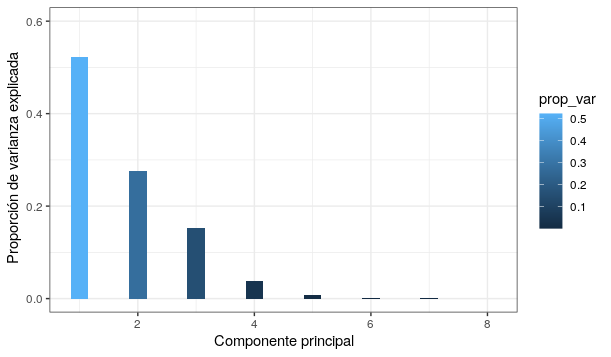
\includegraphics[width=120mm]{imgs/prop-var}
  \caption{Proporción de varianza explicada por cada componente principal}
  \label{fig:prop-var}
\end{figure}

\begin{verbatim}
> cum_var<-cumsum(prop_var)
> ggplot( data = data.frame(cum_var, pc = 1:8),
+         aes(x = pc, y = cum_var ,fill=cum_var )) +
+   geom_col(width = 0.5) +
+   scale_y_continuous(limits = c(0,1)) +
+   theme_bw() +
+   labs(x = "Componente principal",
+        y = "Proporción de varianza acumulada")
\end{verbatim}

\begin{figure}[H]
  \centering
  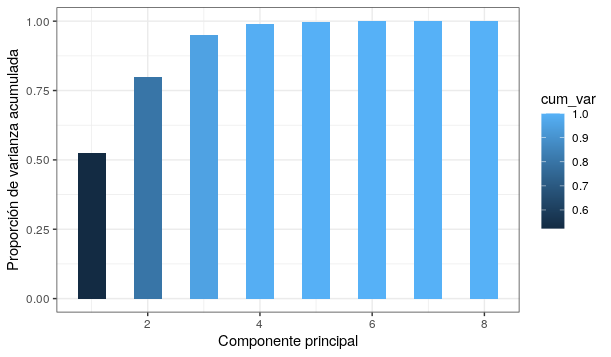
\includegraphics[width=120mm]{imgs/cum-var}
  \caption{Proporción de varianza acumulada por cada componente principal}
  \label{fig:cum-var}
\end{figure}

\pagebreak

\subsection{Selección del número óptimo de componentes principales}

El método que se ha explicado en las sesiones consiste en tomar las
componentes principales cuya varianza sobrepase la media de las
varianzas.
\begin{verbatim}
> round(PCA$sdev^2,4)
[1] 4.1867 2.2123 1.2155 0.3111 0.0565 0.0116 0.0048 0.0014
> round(mean(PCA$sdev^2),4)
[1] 1
\end{verbatim}
En este caso seleccionaríamos las tres primeras componentes principales.

También hemos investigado acerca del
\href{https://en.wikipedia.org/wiki/Elbow_method_%28clustering%29}
  {Método del Codo}.
  Para ello, obtenemos una representación de la varianza acumulada,
  Figura \ref{fig:cum-var}, (también se puede hacer con la explicada,
  pero es algo más complejo de interpretar a simple vista) con puntos
  y líneas.
  \begin{verbatim}
> ggplot( data = data.frame(cum_var, pc = 1:8),
+         aes(x = pc, y = cum_var ,fill=cum_var )) +
+   geom_line(size = 1.5) +
+   geom_point(size=3, fill="black") +
+   scale_y_continuous(limits = c(0,1)) +
+   theme_bw() +
+   labs(x = "Componente principal",
+        y = "Proporción de varianza acumulada")
\end{verbatim}

\begin{figure}[H]
  \centering
  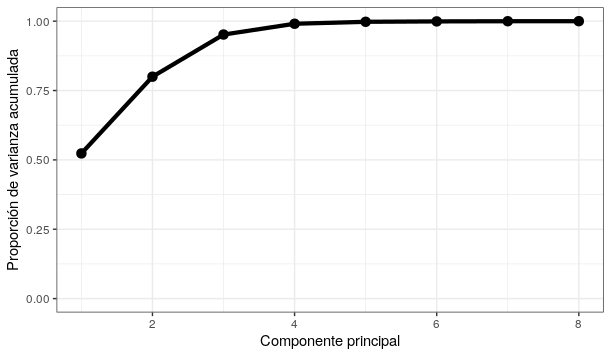
\includegraphics[width=120mm]{imgs/elbow}
  \caption{Proporción de varianza acumulada por cada componente principal}
  \label{fig:elbow}
\end{figure}

También tenemos el codo de la curva para 3 componentes
principales. Las tres primeras componentes principales acumulan una
varianza explicada del 95.18\%.

\pagebreak

\subsection{Representación gráfica de las componentes principales}

Con ayuda del paquete \texttt{factoextra} podemos visualizar para cada
dos de las tres componentes principales la proyección (en el
subespacio correspondiente esas dos componentes) de las instancias y
sus contribuciones a las varianzas. Así como el peso de las variables
en cada componente principal. Lo que podemos identificar en estas
representaciones, también se refleja en la matriz de rotación, Tabla \ref{tab:mat-rot}
(las relaciones entre variables y componentes principales) y en la matriz
de coordenadas de las empresas correspondientes (Tabla \ref{tab:mat-x} a las tres primeras
componentes principales.

\begin{table}[H]
  \centering
  \begin{verbatim}
> t(round(PCA$x[,1:3],3))
         1      2      3      4      5      6      7
PC1 -2.764 -2.193 -1.711  0.456 -1.530 -1.830 -0.934
PC2  1.334  1.036  1.175  2.342 -0.461 -1.005 -1.199
PC3 -0.354 -0.031  2.010 -0.749 -0.497 -0.239 -1.637
         8      9    10     11     12     13 
PC1  2.673  1.892 2.450 -0.121  0.251  3.360
PC2  1.358  0.503 0.248 -2.337 -2.514 -0.479
PC3 -0.383 -0.460 2.115  1.063  0.110 -0.947
\end{verbatim}
  \caption{Matriz con las coordenadas de las proyecciones de las empresas en el subespacio formado por las tres primeras componentes principales.}
  \label{tab:mat-x}
\end{table} \vspace{-5mm}

\begin{verbatim}
> fviz_pca(PCA, axes=c(1,2),
+          alpha.ind ="contrib", col.var = "cos2",col.ind="seagreen",
+          gradient.cols = c("#FDF50E", "#FD960E", "#FD1E0E"),
+          repel=TRUE,
+          legend.title="Distancia")+theme_bw()
\end{verbatim}

\begin{figure}[H]
  \centering
  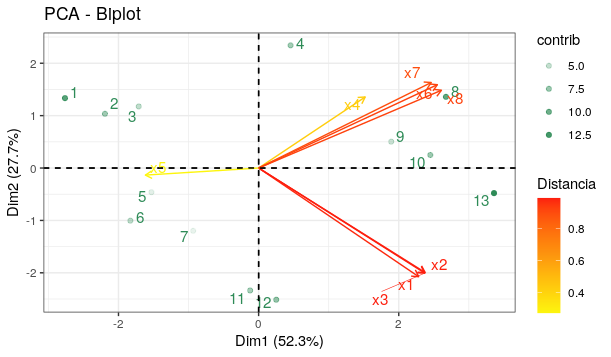
\includegraphics[width=120mm]{imgs/biplot12}
  \caption{Primera y segunda componente principal}
  \label{fig:biplot12}
\end{figure}

\pagebreak

Las instancias que más contribuyen a la varianza son las que aparecen
en verde más oscuro: la empresa 13, la 8 y la 1. Las que menos son las
que aparecen en verde más claro: la empresa 7, la 5, la 9 y la 3. Por
ejemplo, las empresas 11 y 12 tienen una coordenada en la segunda
componente por debajo de -2 y una coordenada cercana a 0 en la primera
componente (como puede comprobarse en la Tabla \ref{tab:mat-x}),
mientras que la empresa 13 tiene una coordenada en la primera
componente cercana a 3 y en la segunda componente cercana a -0.5.

Observamos que respecto a lo que concierne a las dos primeras
componentes principales, las variables X6, X7 y X8 están muy
correladas, igual pasa con las variables X1, X2, y X3. Justamente las
seis variables que acabamos de comentar son las que más contribuyen a
las dos primeras componentes principales. En la Tabla
\ref{tab:mat-rot} vemos que tienen pesos mayores en estas componentes
que las variables X4 y X5. También observamos que los signos de los
pesos concuerdan con la posición de las variables en la parte positiva
o negativa de los ejes. Por último, cabe destacar que la variable X5
queda proyectada muy cerca del eje de la primera componente, por lo
que apenas contribuye a la segunda componente, de hecho en la Tabla
\ref{tab:mat-rot} observamos que su peso es prácticamente nulo.

\begin{verbatim}
> fviz_pca(PCA, axes=c(1,3),
+          alpha.ind ="contrib", col.var = "cos2",col.ind="seagreen",
+          gradient.cols = c("#FDF50E", "#FD960E", "#FD1E0E"),
+          repel=TRUE,
+          legend.title="Distancia")+theme_bw()
\end{verbatim}

\begin{figure}[H]
  \centering
  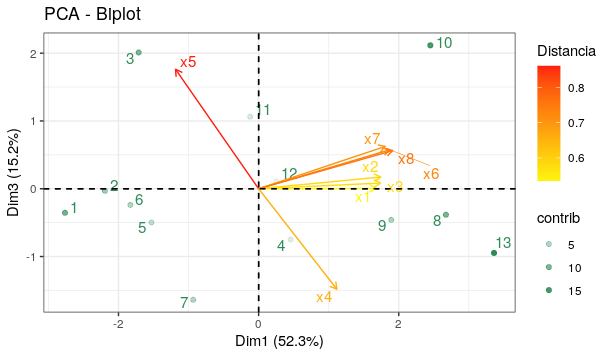
\includegraphics[width=120mm]{imgs/biplot13}
  \caption{Primera y tercera componente principal}
  \label{fig:biplot13}
\end{figure}

\begin{verbatim}
> fviz_pca(PCA, axes=c(2,3),
+          alpha.ind ="contrib", col.var = "cos2",col.ind="seagreen",
+          gradient.cols = c("#FDF50E", "#FD960E", "#FD1E0E"),
+          repel=TRUE,
+          legend.title="Distancia")+theme_bw()
\end{verbatim}

\begin{figure}[H]
  \centering
  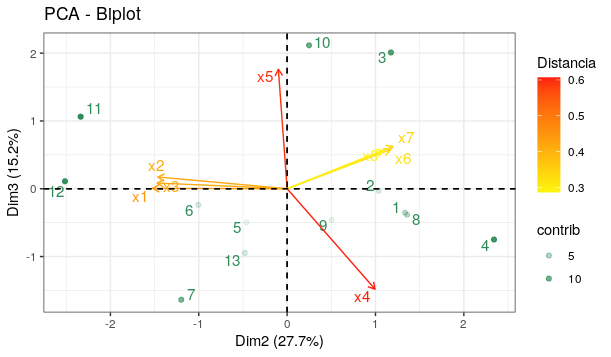
\includegraphics[width=120mm]{imgs/biplot23}
  \caption{Segunda y tercera componente principal}
  \label{fig:biplot23}
\end{figure}
\vspace{-5mm}
Observando las otras dos gráficas, podemos hacer un análisis análogo
al que hemos hecho para la primera. Por destacar alguna idea novedosa,
observamos que las variables X1, X2, X3 aparecen también muy
correladas para estos dos pares de componentes principales; y lo mismo
ocurre con las variables X6, X7, X8. Si nos vamos a la matriz de
correlación al principio de la Sección \ref{sec:acp}, observamos que
entre estas variables existen correlaciones de entre el 96 y el 99\%,
así que es lógico que esto ocurra.

\end{document}
